\documentclass[11pt,a4paper]{article}

% -------------------------
% Packages
% -------------------------
\usepackage[utf8]{inputenc}
\usepackage[T1]{fontenc}
\usepackage{lmodern}
\usepackage{geometry}
\usepackage{microtype}
\usepackage{amsmath,amssymb,amssymb,mathtools}
\usepackage{siunitx}
\usepackage{graphicx}
\usepackage{caption}
\usepackage{subcaption}
\usepackage{hyperref}
\usepackage{fancyhdr}
\usepackage{xcolor}
\usepackage{enumitem}
\usepackage{tikz}
\usepackage{float}
\usepackage{booktabs}
\usepackage{sectsty}
\usepackage{biblatex}

% -------------------------
% Page setup
% -------------------------
\geometry{
  left=25mm,
  right=25mm,
  top=25mm,
  bottom=25mm
}

\pagestyle{fancy}
\fancyhf{}
\lhead{Data Analysis — Final Report}
\rhead{Alexandru Oprea}
\cfoot{\thepage}

% -------------------------
% Title
% -------------------------
\newcommand{\Course}{Data Analysis}
\newcommand{\Assignment}{Replication of Shen et al. (2011)}
\newcommand{\Name}{Alexandru Oprea}
\newcommand{\StudentID}{6153853}
\newcommand{\DateSubmitted}{\today}

\renewcommand{\maketitle}{
  \begin{center}
    {\LARGE\bfseries \Course}\\[6pt]
    {\large\bfseries \Assignment}\\[12pt]
    \begin{tabular}{rl}
      \textbf{Name:} & \Name \\
      \textbf{Matrikel-Nr:} & \StudentID \\
      \textbf{Date:} & \DateSubmitted
    \end{tabular}
    \vspace{10pt}
    \hrule
  \end{center}
}

\newcommand{\question}[1]{\bigskip\noindent\textbf{Question #1.}\quad}
\newcommand{\answer}{\noindent\textbf{Answer.}\quad}
\allsectionsfont{\normalfont\scshape}
\sisetup{detect-all, per-mode=symbol}

% -------------------------
% Document
% -------------------------
\graphicspath{{../figures/}}
\begin{document}

\maketitle
\section{Abstract}

I hereby present a replication of the statistical analysis of quasar emission line properties from the SDSS Data Release 7 catalog of \cite{shen2011} which contains spectroscopic measurements for 105,783 quasars. I replicated figures 13 and 15, showing MgII emission line properties and the 4DE1 eigenvector parameter respectively. After applying quality cuts, I analyzed 42,333 MgII and ~18,000 H$\beta$ quasars. All major correlations were reproduced: FWHM-EW relationship, the Baldwin Effect, the population A/B dichotomy (at FWHM=4000km/s) and the preferential clustering of 8000 radio loud quasars in Population B. I will discuss the methodological challenges encountered during replication, in more detail than in my presentation. Some of the difficulties were quantifying the alpha values (80 discrete values), S/N threshold determination, and binning specifications. All of these things were solved with a mix of guessing, and later on direct correspondence with the original authors. My results validate the complexity of the SDSS DR7 catalog measurements and demonstrate successful open-source replication of large scale spectroscopic analysis. 

\section{Introduction}

\subsection{Quasar Theory}
Quasars are among the most energetic and luminous objects in the Universe. They are powered by the accretion of matter onto supermassive black holes residing at the centers of distant galaxies. With biometric luminosities range from $10^{44}$ to $10^{48}$ erg s$^{-1}$ , quasars outshine their host galaxies by orders of magnitude, making them visible across great distances. Their spectra is characterized by broad emission lines produces in a region of fast moving, photo-ionized gas (Broad Line Region=BLR), which is located within a fraction of a parsec from the central black hole. These emission lines are the main investigation method; the width of a line traces the velocity of the emitting gas, which in turn reflects the gravitational influence of the black hole... while the equivalent width measures the strength of the line relative to the continuum. All of these parameters provide information related to the physical conditions of gas around accreting black holes and that's why we can read them all the way from here.

\subsection{SDSS}
The Sloan Digital Sky Survey (SDSS; York et al. 2000) is one of the biggest spectroscopic survey in the history of astronomy. It systematically observes about one quarter of the sky, collecting spectra over a wavelength range of 3800–9200 Å, at a spectral resolution of R $\sim$ 2000. This survey produced spectra for hundreds of thousands of galaxies, stars, and quasars.  Data Release 7, contains spectra for 929,555 galaxies and 121,363 quasars, with all of the products being available to the public through the SDSS SkyServer and other data repos, making the survey a good model for open science. 

\subsection{S11 Quasar Catalog}

Let's call the Shen et al. (2011) study S11. It presents a comprehensive catalog of spectroscopic measurements for 105,783 quasars from the SDSS DR7. For each quasars S11 measured line widths (FWHM), equivalent widths (EW), continuum luminosities, iron emission strengths and spectral slopes. The measurements were performed for multiple emission lines (mostly for H$\beta$, MgII, and CIV), covering redshift ranges. The catalogue also contains derived quantities including virial black hole mass estimates ( virial mass = mass of a gravitationally bound astrophysical system), Eddington ratios (max luminosity of a celestial body) and radio loudness parameters. Since it's publication, S11 has become a foundation reference in quasar science, having been cited over a thousand times and serving as the basis for a handful amount of black hole demographics and quasar evolution studies. 

\subsection{Motivation}
Reproducing data is a fundamental thing in science. Especially when the analysis is public, using the same data, but maybe with different tools and approaches one is able to validate the analysis. We live in an era where spectroscopic surveys are becoming larger and larger, helping us draw conclusions from hundreds of thousands of objects; that also means we need to verify the statistical results for robustness and investigate any artifacts/ software choices and even undocumented methodological decisions.

In this work, I attempt to replicate two key figures from S11, Figure 13 which shows the statistical properties of MgII emissions line measurements as a 6X6 corner plot; and Figure 15, which shows the projected 4DE1 eigenvector parameter space for $H \beta$ quasars with a radio loud overlay. I have carried the entire analysis in Python using public libraries such as Numpy, Pandas, Matplotlib and Astropy; all in contrast to the IDL-based pipeline for the original work. Below, I am documenting the full methodology, challenges and how they were tackled, including the correspondence with the original authors. 

\section{Theoretical Background}

\subsection{Emission Lines and Broad Line Region}
Quasar spectra displays prominent emission lines superimposed on a power law continuum produced by the accretion disk. These lines arise in the BLR (broad line region), a compact ($\sim 0.1-1pc$), high density ($n_{e}\sim 10^{9-11} cm^{-3}$) region where gas is photo-ionized by the intense ultraviolet radiation field of the central "engine". The thermal and turbulent velocities of the emitting gas, combined with orbital motions around the black hole, produce the characteristically broad line profiles observed with FWHM values ranging from hundreds to tens of thousands of km/s. 

Two of the most important BLR diagnostics are the full width at half maximum (FWHM) of the emission line profile and the equivalent width (EW): 

$$\text{FWHM} = \text{full width of line at } 50\% \text{ of peak flux}$$

$$EW=\int \frac{{F_{cont}-F_{line}}}{F_{cont}}d\lambda$$

The FWHM measures the characteristic velocity of the emitting gas while the EW measures the strength of the line relative to the local continuum. A large EW indicates a stronger emission lane relative to the continuum; its value is sensitive to both the intrinsic line luminosity and the continuum level. 

The spectral slope $\alpha$ is defined through the power-law representation of the quasar continuum:

$$f_\lambda \propto \lambda^\alpha$$
More negative values for $\alpha$ indicate blue (hot) spectra while the positive values indicate redder continua, de to dust reddening or even host galaxy contamination. The typical value for SDSS quasars is $\alpha \approx -1.5$.

The MgII line at 2798Å is of importance because we can access it in the optical for quasars at redshifts $z \sim 0.4-2.22$ and it behaves similarly to $H \beta$ in terms of its virial mass calibration. The $H \beta$ line at 4861 Å for a $z \lesssim 0.8$ provides an additional view of the lower redshift quasar population. 

\subsection{Virial Black Hole Mass Estimation}

A central application of emission line measurements is the estimation of black hole masses using the virial theorem. Under the assumption that BLR gas moves in gravitationally bound orbits around the hole, the mass is: 

$$M_\text{BH} = f \frac{\text{FWHM}^2 \cdot R_\text{BLR}}{G}$$
where $f$ is a dimensionless virial factor that accounts for the geometry and kinematics of the BLR (around a value of 1 usually), and  $R_\text{BLR}$ is of course, the radius of the BLR. This radius cannot be directly measured in most quasars so we estimate it from the continuum luminosity using the empirical R-L relationship established from reverberation mapping campaigns (Kaspi et al. 2000; Vestergaard \& Peterson 2006):

$$R_\text{BLR} \propto L^{0.5}$$
This leads to the single epoch virial mass estimator:

$$M_\text{BH} \propto \text{FWHM}^2 \cdot L^{0.5}$$
Whether or not this is reliable is a matter of the accuracy of the FWHM and luminosity measurements; exactly what S11 aims to do and I am trying to validate. 

\subsection{Baldwin Effect}
The bald twin.. I'm kidding. The Baldwin Effect (Baldwin 1977) is the empirical anti correlation between the equivalent width of broad emission lines and the continuum luminosity of quasars. It was originally discovered for the CIV line in a much smaller sample, and it has been confirmed for multiple emission lines including MgII and $H \beta$ and across several orders of magnitude in luminosity. This is the math behind it: 

$$\log(\text{EW}) = \beta \log(L) + \text{const}, \quad \beta < 0$$

For MgII, the typical slope is $\beta \approx -0.25$, meaning that for every order of magnitude increase in luminosity, the equivalent width decreases by a factor of almost 1.8. Despite nearly 50 years of study the physical origin of the Baldwin Effect is still up to debate. The dilemma is that as luminosity increases, the ionizing photon rate goes up, which makes the BLR gas go to a higher ionizing state and reduces the abundance of ionic species responsible for the emission lines. Another alternative explanation would be: changes in the BLR, the shape of the ionizing spectrum or the geometry of the accretion disk. The Baldwin Effect is relevant to this work since its detection in my independently processed dataset serves as a direct validation of the quality of the luminosity and equivalent with measurements... but at the same time, the definition should be taken with a grain of salt.

\subsection{The 4DE1 Eigenvector and Quasar Population Structure}
Boroson \& Green (1992) performed a PCA of the optical emission line properties of a sample of Palomar (green quasar survey) finding that the first eigenvector (the direction of the maximum variance in the data) was primarily driven by an anti correlation between the strength of iron emission (R$_\text{FeII}$ = EW(FeII)/EW(H$\beta$)) and the width of the $H \beta$ line. This eigenvector (dubbed as EV1) and its extension to other wavelengths make what is now known as the Four Dimensional Eigenvector 1 scheme (Sulentic et al. 2000).

In the 4DE1 space, quasars are classified into two broad populations based on their $H \beta$FWHM:
\begin{itemize}
    \item Population A: FWHM $(H \beta)<4000kms^{-1}$. These objects tend to have stronger iron emission (high R$_\text{FeII}$), are preferentially radio quiet and are thought to be accreting at relatively high Eddington ratios.
    \item Population B:  FWHM $(H \beta)\geq4000kms^{-1}$. These objects tend to have weaker iron emission  (low R$_\text{FeII}$), are radio loud and associated with lower Eddington ratio accretion and possibly geometrically thicker accretion disks.
\end{itemize}

\subsection{Radio Loudness}
Radio Loudness is quantified by the radio to optical flux ratio:

$$R = \frac{f_{5\,\text{GHz}}}{f_{4400\,\text{Å}}}$$

Quasars with R>10 are classified as radio loud and thought to launch powerful relativistic jets that produce synchrotron radiation (intense electromagnetic radiation) across the radio spectrum. Radio loud quasars constitute approximately 10\% of the overall quasar population Their preferential location in Population B of the 4DE1 parameter space suggests a connection between jet production and the accretion mode: the broader-line, low iron regime of Population B may favor conditions (like geometrically thick disks) that favor jet launching. In the SDSS DR7 catalog, radio loudness is available as the pre computed parameter RL for objects detected in the FIRST survey with 9,399 quasars having positive radio detections.

\section{Data and Methods}
\subsection{Catalog Structure}
The primary dataset for the SDSS DR7 quasar catalog of S11 is available to the public through the VizieR database. It is distributed as a fixed-width ASCII table that is accompanied by a machine readable column description, which we can think of as the "key" that opens the data file (ReadMe). It contains 105,783 rows with one row dedicated per quasar... and 180 columns covering spectroscopic measurements, derived quantities and auxiliary data. I have accessed this catalog using the Astropy ASCII interface and converted it to a pandas DataFrame for subsequent analysis. 

The key columns used in this work are summarized in Table 1. Measurements for MgII are available for 85,507 quasars (those with redshift placing the line in the SDSS spectral window), while the $H \beta$ measurements are available for 22,715 quasars (lower redshift objects). Radio loudness (RL) is available for all entries with negative sentinel values (RL=-1) which indicates non detections.


\begin{table}
\centering
\caption{Key columns used from the Shen et al. (2011) catalog.}
\label{tab:catalog_columns}
\begin{tabular}{llcc}
\hline
\hline
Column & Description & Units & N valid \\
\hline
W(BMgII) & MgII broad component FWHM & km~s$^{-1}$ & 85,507 \\
EWBMgII & MgII broad component EW & \AA & 85,507 \\
logL3000 & Continuum luminosity at 3000~\AA & log(erg~s$^{-1}$) & 85,507 \\
FeMgII & FeII EW in MgII region & \AA & 85,507 \\
alphMgII & Continuum slope (MgII region) & --- & 85,507 \\
SN(MgII) & Median S/N per pixel & --- & 85,507 \\
W(BHb) & H$\beta$ broad component FWHM & km~s$^{-1}$ & 22,715 \\
EWBHb & H$\beta$ broad component EW & \AA & 22,644 \\
EWFeHb & FeII EW in H$\beta$ region & \AA & 20,810 \\
logL5100 & Continuum luminosity at 5100~\AA & log(erg~s$^{-1}$) & 23,093 \\
RL & Radio loudness parameter & --- & 105,783 \\
FIRST & FIRST survey detection flag & --- & 9,399 \\
\hline
\end{tabular}
\end{table}

\subsection{Quality Cuts}
\subsubsection{MgII Sample}
My initial quality cut for the MgII sample was derived from a thorough reading of S11 and standard practice (assumption and playing around):

\begin{itemize}
    \item Valid measurements: logL3000 > 0, W(BMgII) > 0, EWBMgII > 0, FeMgII > 0
    \item Physical range: 5 < W(BMgII) < 20,000 $kms^-1$
    \item Physical range: 500 < EWBMgII < 500 Å
    \item Physical range: 42 < logL3000 < 48
    \item Data quality: SN(MgII) > 3 (as stated in the paper)
\end{itemize}

The initial selection returned 81,316 quasars which is twice the sample size that was used for Figure 13. To determine this discrepancy, I have systematically tested alternative S/N thresholds. The results were summarized in Table 2. Something like S/N > 10 yields 42,333 quasars which comes close to their sample size of almost 44 k. So I therefore adopted this value for the MgII quality cut. This sound to noise ratio discrepancy was not documented in the S11. I think it is common practice in large survey to apply more cuts for key figures (to make them pretty) than the minimum threshold quoted for the overall catalog within the paper. 

\begin{table}[H]
\centering
\caption{MgII sample sizes as a function of the S/N threshold, after all other quality cuts.}
\label{tab:sn_thresholds}
\begin{tabular}{ccl}
\toprule
S/N threshold & N quasars & Notes \\
\midrule
$>$ 3  & 81,316 & As stated in S11, too many \\
$>$ 5  & 71,213 & Still too many \\
$>$ 7  & 59,818 & Still too many \\
$>$ 10 & 42,333 & Matches S11 Figure 13 \checkmark \\
$>$ 15 & 18,738 & Too few \\
\bottomrule
\end{tabular}
\end{table}


\subsubsection{$H\beta$ Sample}
For the $H \beta$ sample used in Figure 14, I have applied the following cuts:
\begin{itemize}
    \item Valid measurements: W(BHb)>0, EWBHb>0, EWFeHb>0
    \item Physical range: 1000<W(BHb)<20,000 km/s
    \item $R_{{FeII}}$ range: 0 < $R_{Fe}$<3.5
    \item Data quality: SN(Hb) > 3
\end{itemize}

These cuts return 18,000 quasars which is consistent with the $H \beta$ sample in S11. The lower S/N threshold (3 vs 10) is somewhat appropriate for $H\beta$ as the smaller total sample would be severely reduced by stricter cuts.

\subsubsection{Radio-loud subsample}

For this radio-loud quasars I only needed to use the RL column. Based on the literature, a radio-loud quasar has an RL>10. This gave 8,256 RL quasars out of which only 1410 fall within the $H \beta$ quality cut sample used for Fig 15, which is almost 7.5\% of the $H \beta$ sample.

\subsection{Variable Definitions and Operations}

In order to reduce the dynamic range of the data and facilitate visual comparison, I had to transform most variables to a log value prior to the analysis: 

$$\log\text{FWHM} = \log_{10}[W(\text{BMgII})]$$
$$\log\text{EW} = \log_{10}[\text{EWBMgII}]$$
$$\log\text{EWFe} = \log_{10}[\text{FeMgII}]$$
Other variables were already provided in the logarithmic form. The spectral slope $\alpha$ and the median S/N were preserved... and lastly, the iron ratio for Fig 15 was computed as

$$R_\text{FeII} = \frac{\text{EWFeHb}}{\text{EWBHb}}$$

\subsection{Pipeline and Visualization}

So, for Figure 13 I had to stick to the following steps: 

\begin{enumerate}
    \item Loaded the catalog and converted it to a pandas DataFrame.
    \item Applied MgII quality cuts (S/N>10) which yielded 42,333 quasars.
    \item Log transformation (where necessary) 
    \item  For each pair of variables $(i,j)$ with $j<i$:
    \begin{itemize}
        \item Clipped the data to 1st-99th percentile in order to remove the outliers
        \item Constructed 2D histograms with bin resolution $\Delta=0.1$ for log quantities and  $\Delta=2$ for S/N (*)
        \item Computed contour levels as 5-7 linearly spaced values between 20\% and 90\% of the histogram maximum
        \item Overlay contours on a log scale density map
    \end{itemize}
    \item For the diagonal panels I had to construct a 1D histogram with the same bin resolution
    \item Everything was then wrapped in a 6X6 lower triangular corner plot
\end{enumerate}

And for Figure 15, the pipeline was:

\begin{enumerate}
    \item Apply $H \beta$ quality cuts, which returned around 18,000 quasars. 
    \item Computed $R_{FeII}$
    \item Identified the radio loud subset (again, values for RL above 10)
    \item Constructed 2D histograms for all quasars and RL subset separately 
    \item Plotted contours with black solid lines for all quasars and the red dashed ones for radio-loud
    \item Added a Population A/B boundary at FWHM=4000 km/s
\end{enumerate}

The binning specifications had to be clarified so I have emailed Dr. Yue Shen (main author of S11). He had told me to set the bin resolutions in (x), contour levels equally spaced in linear scale and to remove the Gaussian smoothing that I initially had.
I was still skeptical after this communication since our figures were still very different. I have used Matplotlib to plot everything, but in S11 they had used IDL and used contours on a white background without filled density. While they differ aesthetically, they come close in conveying the same scientific information. I chose to retain the filled density visualization because it makes density gradients more apparent on a high resolution display. It's still information that can be used at the end of the day. I blame it on the fact that astropy was not out during that time and most astrophysicists had to make do with IDL as they were skeptical of switching to python.

\section{Results}

\subsection{MgII statistical properties}
Figure \ref{fig:mgii_corner} shows my replication of Figure 13 from S11, displaying pairs of statistical properties of six MgII related quantities for the 42,333 quasars that were cut off after the quality assessment. The distribution of log FWHM(MgII) peaks at approximately log FWHM  $\approx$ 3.6 (corresponding to FWHM $\approx$ 4000 km s$^{-1}$), with a histogram peak of 11475, is in agreement with the peak of approximately 12000 shown in S11. The distribution is approximately log-normal from $\sim$ 2.7 to $\sim$ 4.3 in log units after quality cuts. 

\begin{figure*}
\centering
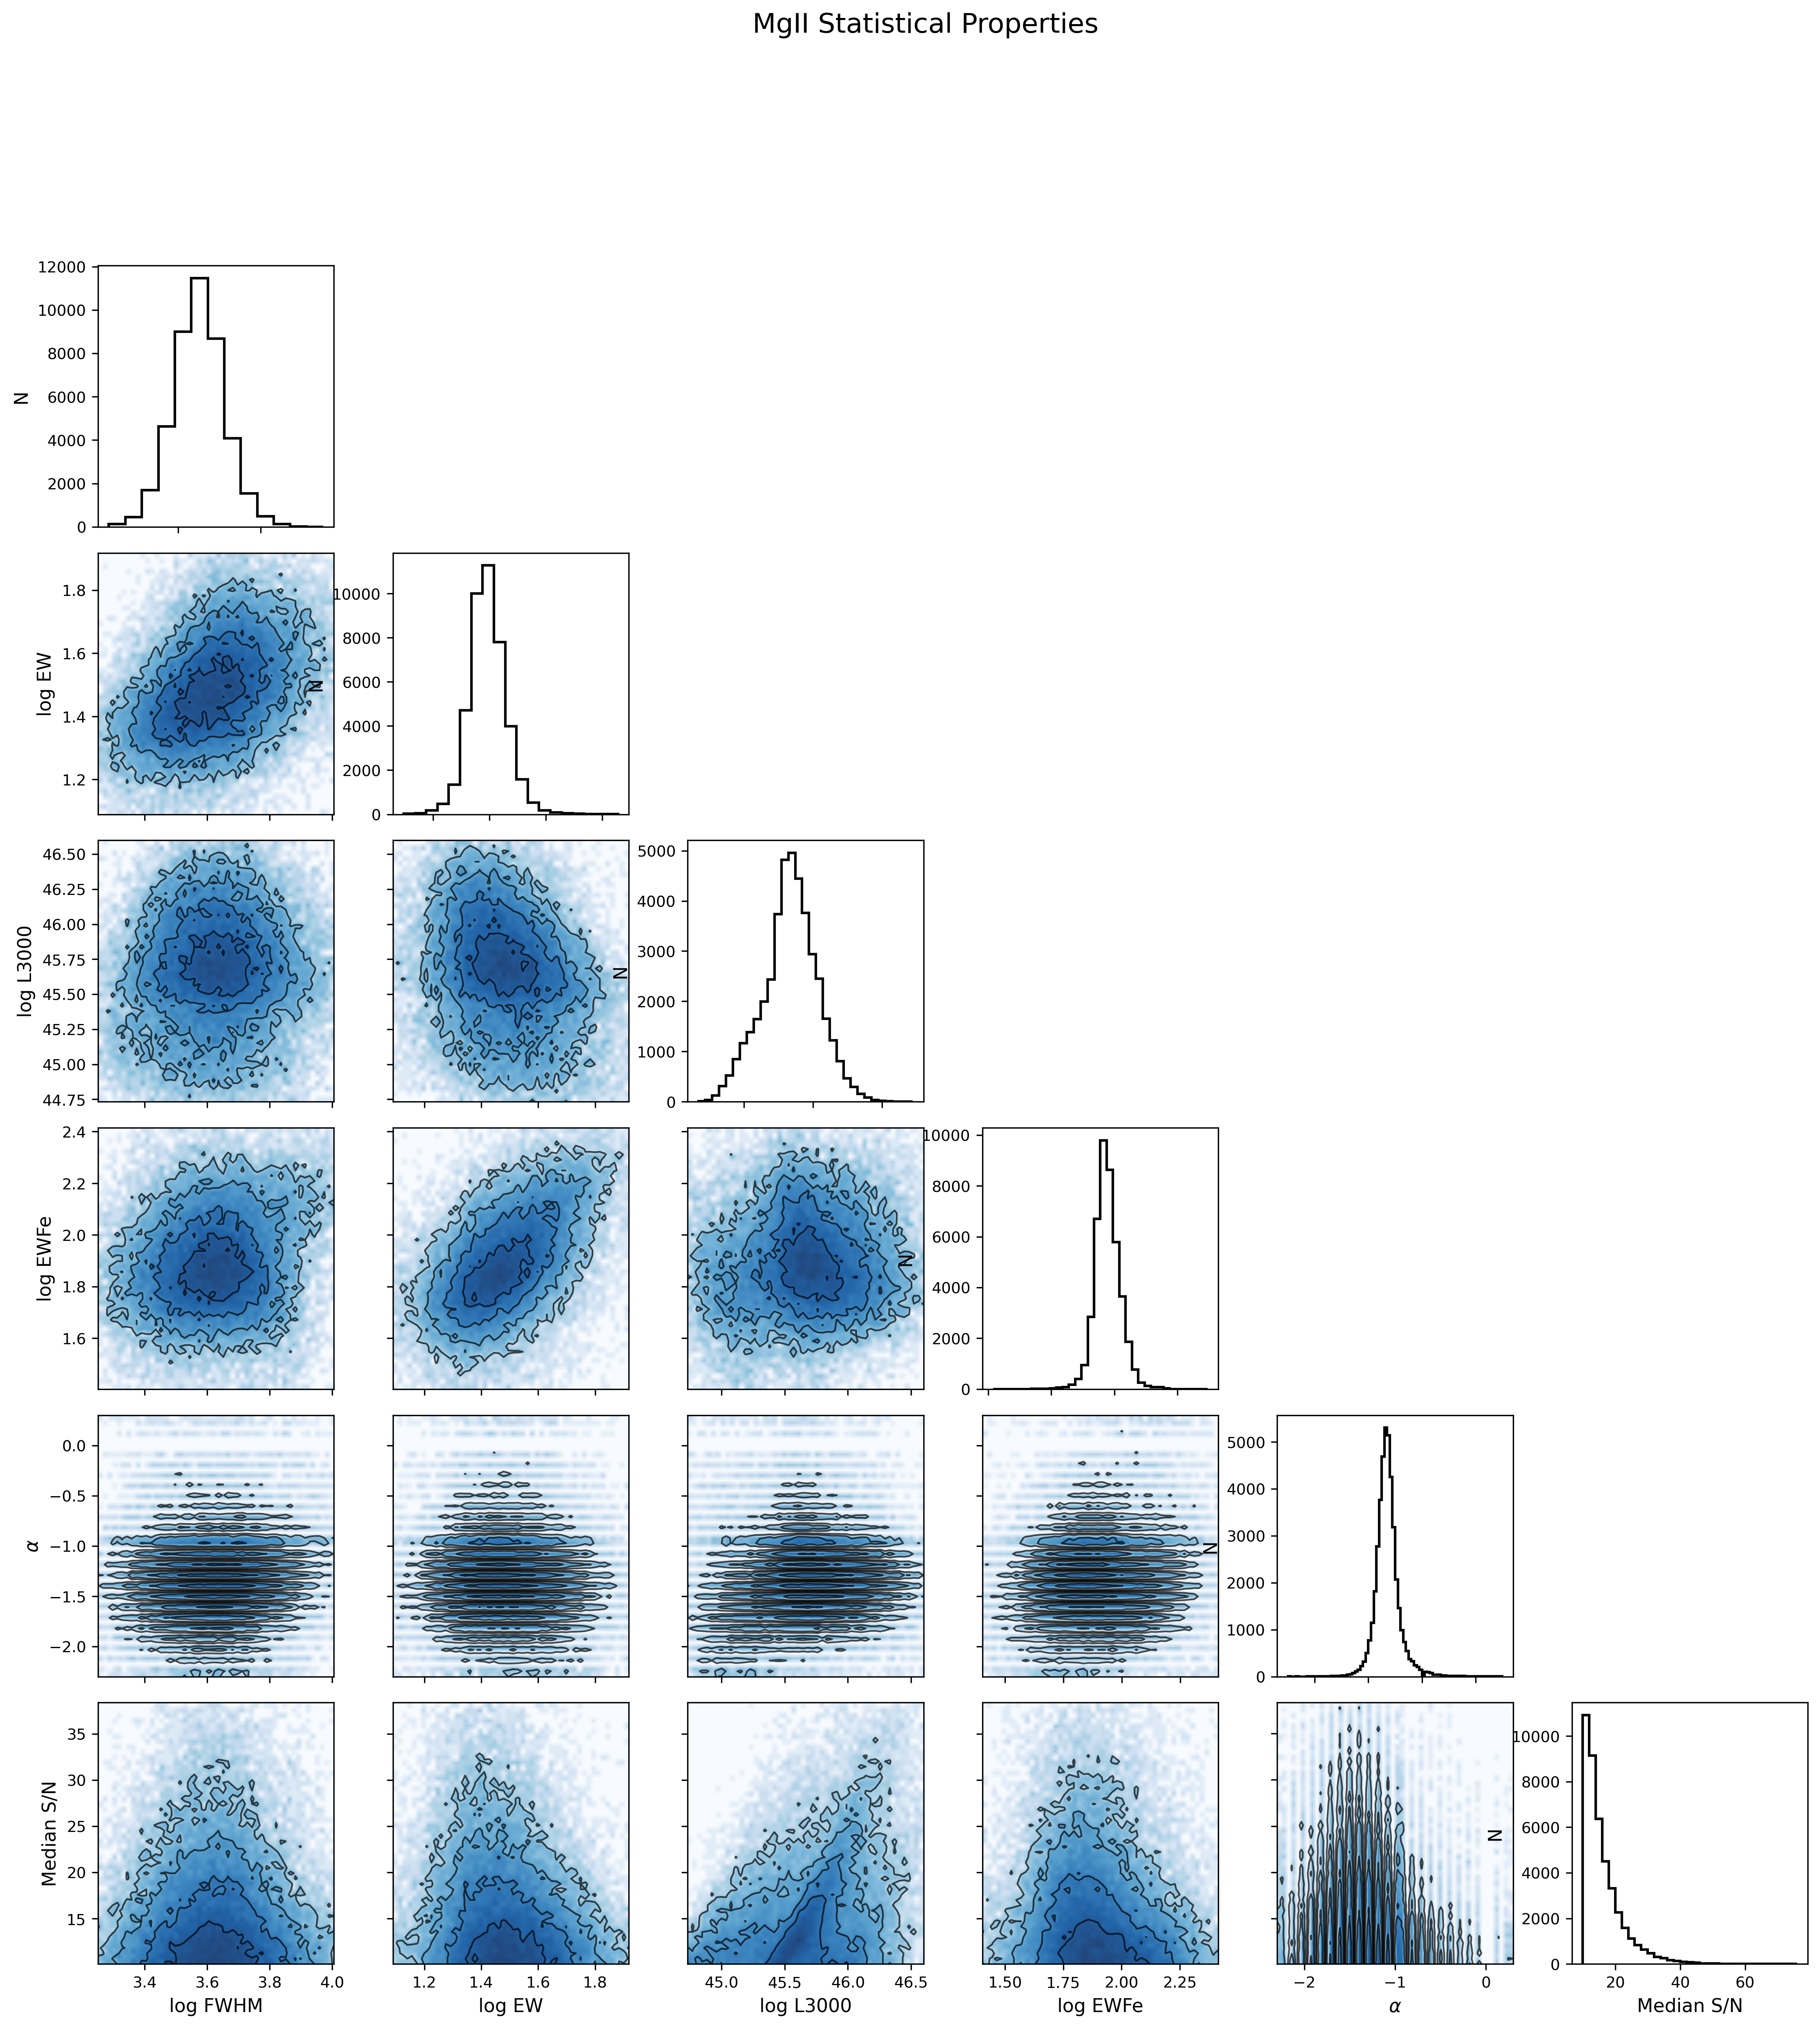
\includegraphics[width=0.95\textwidth]{fig13_MgII_final.png}
\caption{Statistical properties of MgII emission line measurements for 42,333 
SDSS DR7 quasars after quality cuts (S/N $>$ 10). The diagonal panels show 
1D histograms of each variable; off-diagonal panels show 2D density distributions 
with contour overlays. Key correlations are visible: the FWHM-EW positive 
correlation (panel [2,1], $r \approx +0.6$), the Baldwin Effect anti-correlation 
between luminosity and equivalent width (panel [3,2], $r \approx -0.3$), and 
the quantization of the spectral slope $\alpha$ into 80 discrete values 
(horizontal striations in row 5).}
\label{fig:mgii_corner}
\end{figure*}


The log EW distribution peaks at log EW $\approx$ 1.6 (EW $\approx$ 40 Å) with a peak count of 11276, again, very closely matching S11. The distribution is more symmetric than the previous one, showing a narrower range.

The log L3000 distribution spans approximately 43.7 to 47.4 in log(erg s$^{-1}$), with a peak at log L $\approx$ 45.5. This distribution is broader, nearly by four orders of magnitude, and it reflects the wide range of the accretion rates and black holes masses that were sampled by the SDSS at redshifts $z \sim$ 0.4-2.2.

The log EWFe distribution is broad and more asymmetric than the rest of the parameters, with a peak (i would not even call it a peak, let's call it a tendency) near log EWFe $\approx$ 2.0 and a long tail toward both higher and lower values. This matches the known diversity in iron emission properties across quasars which is closely linked to the 4DE1 eigenvector structure (Boroson \& Green 1992).

The spectral slope $\alpha$ distribution, the thing that made most of my work insufferable, exhibits a sharp peak near $\alpha \approx$-1.4, which matches the typical blue quasar continuum. A thing that stands out in this distribution, something that you can't miss in those 2D panels is the presence of almost 80 discrete values that are separated by $\Delta \alpha =0.1$. This quantization arises from the measurement precision of the continuum slope fitting in moderate S/N spectra, which I will discuss further.

The S/N distribution shows a sharp lower cutoff at S/N of almost 10 (which is imposed by my quality cut), with a peak near S/N $\approx$ 12 and a long tail that extends to S/N $\sim$ 75 for the brightest quasars. 


\textbf{FWHM-EW Correlation}: The panel showing log FWHM vs log EW (panel 2.1) indicates a strong correlation with a Pearson coefficient of r$\approx$ +0.6. Typically, quasars with broader lines have stronger lines. This is related to the fact that the accretion rate onto the central black hole drives the gas to higher velocities(an increase in FWHM) while it also increases the gas density and covering factor in the BLR (which then increases the EW). This relationship was documented by Dong et al. (2009), mostly for MgII and we can assume that it s is confirmed for all 42,333 objects.

\textbf{The Baldwin Effect}: In panel [3,2], we can see the relationship between log L3000 and log EW which is an anti-correlation with an r$\approx$ -0.3 (indicating the Baldwin Effect). So, Quasars with higher continuum luminosities systematically exhibit weaker MgII emissions relative to their continua. The slope $\beta \approx$-.025 is consistent with literature values for MgII/ Over the two orders of magnitude in luminosity spanned by our sample, the typical EW decreases from almost 60Å at $L_{3000} \sim 10^{44}$ erg s$^{-1}$ to almost 30 Å at $L_{3000} \sim 10^{46}$ erg s$^{-1}$.

\textbf{FWHM-Luminosity}: in panel [3,1] we see a somewhat weak correlation between log FWHM and log L3000 with larger scatter at all luminosity. I was somewhat expecting this since luminosity is dependent on both a black hole's mass and Eddington ratio, while FWHM primarily traces mass. The diversity of Eddington ratios across the population produces scatter that washes out any underlying mass-luminosity relation.

\textbf{Fe correlation}: The iron equivalent width shows a moderate positive correlation with MgII EW in panel [4,2] with an r $\approx$ +0.4, pointing at similar gas density and ionization conditions that support both emissions at the same time. The weak negative correlation between log EWFe and log FWHM in panel [4,1] is related to the Eigenvector 1 pattern; quasars with broader lines (population B) tend to have weaker iron emission while narrow line quasars (population A) have stronger iron.

\textbf{Alpha Panels}: All panes that involve $\alpha$ show weak correlations and a lot of striations. After investigating WHY these striations are present, I figured that is because only 80 discrete values of $\alpha$ exist in the catalog (separated by $\Delta \alpha=0.1$), creating horizontal bands in the 2D density maps. This is present in both my figures and the S11 ones, though it is more visually prominent in my high-res display (not trying to sound entitled but IDL is primitive and low quality) than in the printed version of the paper. The weak correlations between $\alpha$ and all other variables suggest that the continuum slope is largely independent of the emission line properties in this sample.

\textbf{S/N correlations}: The bottom row of pans shows positive correlations between S/N... and most other variables that are more apparent when tied to luminosity (panel [6,3]). This is an observational effect; brighter quasars produce more photons and therefore have a higher S/N in their spectra. This is not a physical correlation and I will not account for it when interpreting luminosity dependent results. 

\subsection{4DE1 Parameter Space}

Figure \ref{fig:4de1} shows my replication of Figure 15 of S11 which shows the 4DE1 eigenvector parameter space: FWHM(H$\beta$) versus R$_\text{FeII}$ = EW(FeII)/EW(H$\beta$) for almost 18,000 H$\beta$ quasars. The black solid contours show the distribution of all quasars meanwhile the red dashed contours show the radio-loud subsample (RL>10).

\begin{figure}
\centering
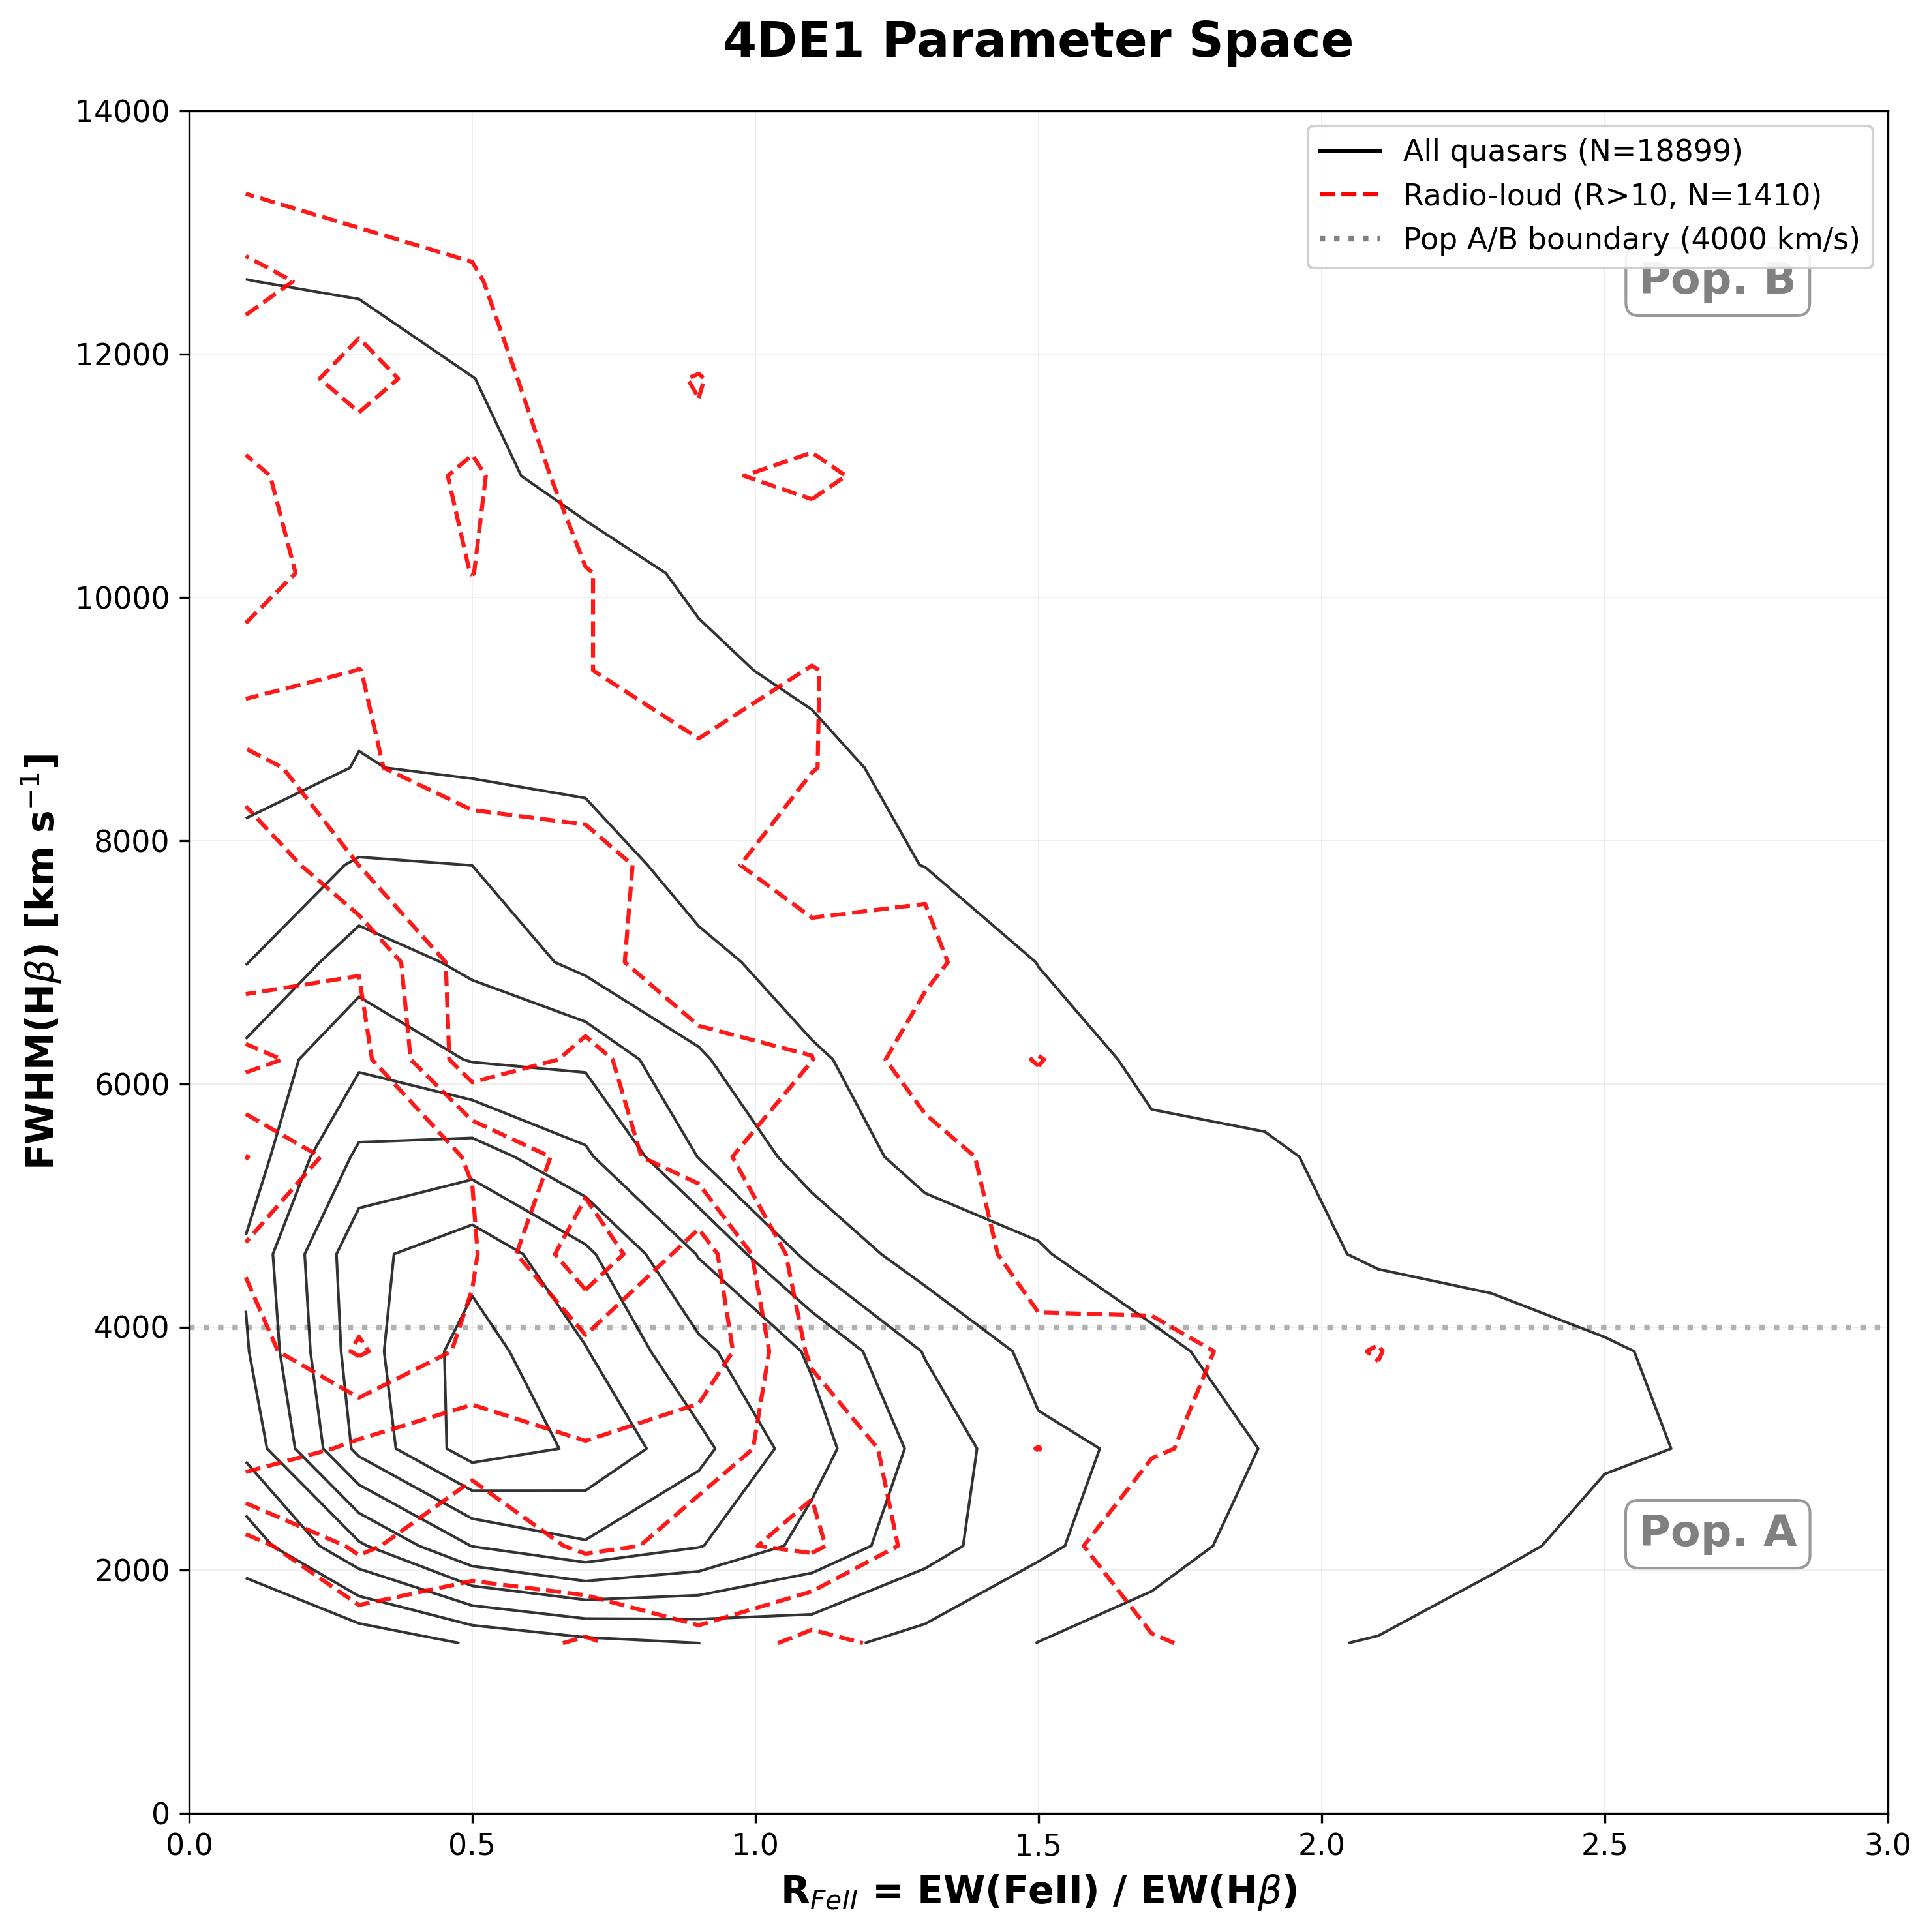
\includegraphics[width=\columnwidth]{fig15_4DE1_with_radio.png}
\caption{The 4DE1 eigenvector parameter space showing FWHM(H$\beta$) versus 
R$_{\rm FeII}$ = EW(FeII)/EW(H$\beta$) for 18,899 H$\beta$ quasars. Black 
solid contours show all quasars; red dashed contours show 1,410 radio-loud 
quasars (RL $>$ 10). The gray dotted line at FWHM = 4000~km~s$^{-1}$ marks 
the Population A/B boundary. Radio-loud quasars cluster preferentially in 
Population B (67.7\% vs.\ 51.8\% overall), with an enrichment factor of 1.31$\times$.}
\label{fig:4de1}

\end{figure}

The distribution in 4DE1 space shows a clear bimodal structure, naturally divided by the boundary at FWHM(H$\beta$)= 4000 km/s. Population A(FWHM < 4000 km/s) quasars cluster at intermediate to high $R_{FeII}$ values, while Population B(FWHM $\geq$ 4000 km/s) quasars extend to lower $R_{FeII}$ values. 

The black contours reproduce the overall shape of the S11 Figure 15 distribution in both the location of the density peak and the extent of the tails.

When addressing red line contours (radio loud quasars) we can see that they have a preference of clustering in Population B with an offset toward higher FWHM relative to the overall sample. About 67.7\% of the radio loud quasars in the H$\beta$ sample fall in Population B compared to 32.3\% in population A which indicates that radio-loud are 1.31x more likely to be in Pop B. This confirms previous studies that indicate that radio loud AGN preferentially occupy the broader line, lower iron regime of the 4DE1 parameter space (Sulentic et al. 2000; S11). The physical interpretation is that the accretion conditions characteristic of Population B indicate different jet emissions. 

\section{Discussion}

The overall replication of the results from S11 was quantitatively successful. Sample sizes agree within let's say 4-10\% and same goes for the peaks of histograms, while preserving the overall shapes. Every major correlation that was identified in the S11 study was also reproduced by my independent analysis: FWHM-EW relationship, the Baldwin Effect, the 4DE1 population structure and the radio loud clustering in Population B. 

When it comes to the challenges I faced, the most significant one was the discrepancy between the sample size implied by the stated S/N threshold (S/N > 3, yielding 81,316 quasars) and the sample size shown in S11 Figure 13 which was of almost 44,000. I had to systematically test these thresholds and I have found out that a S/N>10 produces the sample size. This indicates that S11 applied a more stringent quality cut for Figure 13 than the minimum threshold quoted for the overall catalog which feels a bit bitter. A lot of these big studies seem to not document all of the changes to their dataset. I had to email Dr. Yue Shen that then confirmed binning and visualization specifications but did not really resolve the S/N threshold question entirely. So, yeah, in the end it still had to be a trial and error test from my part.

Methods sections in published papers just summarize than exhaustively document all of their choices. This gap is subtle but it can really affect results one trying to replicate them.

My least favorite part was working with the alpha values, because they displayed horizontal striations throughout the alpha panes of Figure 13. I had to accept that this came from the discrete value of the $\alpha$ measurements. I had to inspect the catalog and find out that this variable has 80 unique values between [-5,+3] spaced at intervals of $\Delta\alpha = 0.1$. This wasn't a plotting artifact after all; it just meant that the slope fitting procedure produces estimates rounded to the nearest 0.1. I investigate the correlation with S/N again, and I noticed that at S/N>10 six of the most extreme alpha values (in the range -4.9 to -4) are removed because they are only populated by low S/N objects, which then creates those striations you see on the plot. They are definitely more apparent in my feature than in S11 but the underlying features (i.e shape) is identical in both.

When it comes to physical interpretation, the successful replication of all major correlations in S11 confirms the physical picture of quasar diversity that has emerged from large scale spectroscopic surveys. The FWHM-EW relationship demonstrates that gas velocity and covering in the BLR are tied, probably through a dependence on the accretion rate. The Baldwin Effect confirms the role of the ionization parameter in setting the relative strength of broad emission lines across orders of magnitude and luminosity. The 4DE1 structure confirms two broad quasar populations with distinct emissions and the preference for loud quasars in Population B is probably linked to jet production and accretion rate.

\section{Conclusion}

I have successfully replicated two figures of Shen et al. (2011), reproducing the statistical properties of MgII emission line measurements and the 4DE1 eigenvector parameter space for SDSS DR7 and I can draw the following main conclusions:
\begin{itemize}
    \item After applying quality cuts such as a median S/N>10 threshold, I recovered 42,333 MgII quasars within 4\% of the S11 sample, with histogram peak counts matching the paper with the same percentage. 
    \item All major correlation in Figure 13 were reproduced, with a clean similarity in the shape of the 2D plots. 
    \item The spectral slope $\alpha$ is quantized to 80 discrete values in the catalog, producing characterizing horizontal striations in the 2D density maps. This is real data having measurement precision limits and not a plotting artifact.
    \item  The 4DE1 parameter space (Figure 15) clearly reproduces the Population A/B dichotomy at FWHM(H$\beta$)=4000km/s, and the radio loud subsample (RL>10, N$\approx$ 8000) is confirmed to cluster preferentially in Population B, which supports the connecting between jet producing and accretion mode.
    \item The effective S/N threshold used in S11 for Figure 13 is a different one than what was stated in the paper.
    \item Direct author correspondence was necessary to resolve these ambiguities in binning specification and contour calculation, but in the end it was not a given; I still had to go through the process of trial and error.
\end{itemize}

Finally, my results confirm that the SDSS DR7 quasar catalog measurements are complex and reproducible using modern open source tools. The complete analysis code is available in the zip file, and not in the Appendix as it's a bit too much.


\printbibliography



\bigskip
\noindent\textit{End of submission.}

\end{document}
